\chapter{Lösungsansätze für Vier Gewinnt}

\section{Optimale Strategien}
Die spieltheoretische Analyse von „Vier Gewinnt“ offenbart eine Reihe von strategischen Prinzipien und optimalen Spielweisen, die das Verständnis dieses Spiels vertiefen und präzise Strategien für Spieler ermöglichen. Diese Erkenntnisse basieren sowohl auf grundlegenden strategischen Prinzipien als auch auf fortgeschrittenen taktischen Elementen, die im Verlauf des Spiels entscheidend sind.

Zu den grundlegenden strategischen Prinzipien gehört vor allem die Bedeutung der Startposition. Es ist nachgewiesen, dass der erste Spieler bei perfektem Spiel immer gewinnen kann, vorausgesetzt, er wählt die optimale Eröffnung. Diese besteht darin, den ersten Stein in die mittlere Spalte zu setzen. Diese Eröffnung bietet die beste Kontrolle über das Spielfeld und erhöht die Möglichkeiten für offensive und defensive Züge in den folgenden Spielphasen. Züge in die benachbarten Spalten (d.h. die zweite oder sechste Spalte) führen bei optimaler Spielweise beider Spieler hingegen zu einem Remis. Alle anderen Eröffnungszüge gelten als suboptimal und führen bei perfektem Gegenspiel unweigerlich zur Niederlage des ersten Spielers.

Ein weiteres zentrales Prinzip ist die Zentrumsbeherrschung, die eine essenzielle Rolle spielt. Die Kontrolle der mittleren drei Spalten (insbesondere der Spalten c, d und e) ist von strategischer Bedeutung, da sie die größten Möglichkeiten für horizontale, vertikale und diagonale Gewinnreihen bieten. Besonders die Spalten b und f – die zweite und vorletzte Spalte – besitzen ebenfalls strategisches Potenzial, da ohne sie keine vollständigen diagonalen oder horizontalen Viererreihen aufgebaut werden können. Diese Kontrolle ist nicht nur wichtig für den eigenen Spielaufbau, sondern auch, um den Gegner in seiner Strategie einzuschränken.

Neben diesen grundlegenden Prinzipien kommen im Verlauf des Spiels auch fortgeschrittene taktische Elemente ins Spiel. Eine der wichtigsten Taktiken ist die Kontrolle über sogenannte Zugzwang-Situationen. Dabei handelt es sich um Spielsituationen, in denen der Gegner durch geschicktes Manövrieren gezwungen wird, einen Zug zu machen, der seine eigene Position verschlechtert. Diese Situationen sind besonders am Ende des Spiels entscheidend, wenn nur noch wenige Felder verfügbar sind und der Druck auf beide Spieler steigt. Ein weiteres taktisches Element sind Fallenkombinationen, bei denen der Gegner durch geschickte Kombinationen von Drohungen in eine Falle gelockt wird. Besonders effektiv sind sogenannte Doppelfallen, bei denen zwei gleichzeitige Drohungen erzeugt werden, die der Gegner nicht beide blockieren kann. Ebenfalls relevant sind Auffüllfallen, bei denen ein Spieler den Gegner durch Mangel an freien Feldern zwingt, einen entscheidenden Stein unter eine vorbereitete Blockfalle zu setzen.

Die spieltheoretische Analyse von „Vier Gewinnt“ wurde durch mathematische und computerbasierte Methoden weiter vertieft. Unabhängig voneinander gelang es zwei Forschern, eine vollständige Lösung für das Spiel zu finden. Victor Allis entwickelte 1988 einen speziellen Regelsatz zur systematischen Analyse des Spiels, während James D. Allen 1990 Computerprogramme einsetzte, um das Spiel vollständig zu berechnen. Beide kamen unabhängig voneinander zum gleichen Ergebnis: Der erste Spieler kann bei optimaler Spielweise und einer Eröffnung in der Mittelspalte das Spiel immer gewinnen. Diese Erkenntnis hat nicht nur wissenschaftliche Relevanz, sondern bildet auch die Grundlage für die Entwicklung von Algorithmen, die in Computerprogrammen oder Robotersystemen eingesetzt werden, um das Spiel optimal zu spielen.


	\begin{center}
		\setlength{\arrayrulewidth}{1mm}
		\setlength{\tabcolsep}{10pt}
		\renewcommand{\arraystretch}{1.5}
		\begin{tabular}{|>{\columncolor[gray]{0.9}}c|c|c|c|>{\columncolor[gray]{0.8}}c|c|c|}
			\hline
			& & & \cellcolor[gray]{0.9} & & & \\ \hline
			& & & \cellcolor[gray]{0.9} & & & \\ \hline
			& & & \cellcolor[gray]{0.9} & & & \\ \hline
			& & & \cellcolor[gray]{0.9} & & & \\ \hline
			& & & \cellcolor[gray]{0.9} & & & \\ \hline
			1 & 2 & 3 & 4 & 5 & 6 & 7 \\ \hline
		\end{tabular}
	\end{center}
	
	\subsection*{Mögliche Startpositionen und Spielausgänge}
	
	\textbf{1. Startposition 4 (mittlere Spalte)}
	Wenn der erste Spieler in die mittlere Spalte setzt, hat er einen nachgewiesenen Vorteil und kann bei perfektem Spiel gewinnen. Diese Eröffnung maximiert die Kontrolle über das Spielfeld.
	
	\textbf{2. Startpositionen 3 oder 5 (benachbarte Spalten zur Mitte)}
	Ein Zug in die Spalte 3 oder 5 führt bei optimalem Spiel zu einem Remis, da der zweite Spieler durch eine Kombination aus Zentrums- und Blockstrategien den Sieg verhindern kann.
	
	\textbf{3. Startpositionen 1, 2, 6 oder 7 (äußere Spalten)}
	Züge in die äußeren Spalten gelten als suboptimal. Der erste Spieler verliert bei perfektem Gegenspiel des zweiten Spielers, da diese Positionen weniger Kontrolle über das Zentrum und die Gewinnlinien bieten.
	
	Diese Analyse zeigt, wie wichtig die Wahl der Startposition für den weiteren Spielverlauf ist. Der erste Zug in die Mitte eröffnet dem Spieler die besten Chancen, während Züge in die äußeren Spalten zu deutlichen Nachteilen führen können.

\section{Heuristische Ansätze}

Die Bewertung von Positionen auf dem Spielfeld ist ein zentraler heuristischer Ansatz bei der Strategieentwicklung für Vier Gewinnt. Dieser Ansatz zielt darauf ab, den strategischen Wert jeder Position systematisch zu analysieren und darauf aufbauend optimale Züge zu planen.

Die dargestellte Tabelle veranschaulicht die strategische Bewertung jedes Spielfelds im Spiel „Vier Gewinnt“. Jedes Feld erhält einen numerischen Wert, der angibt, wie viele mögliche Viererreihen dieses Feld beeinflussen kann. Ein Zug auf ein Feld mit einem höheren Wert ist in der Regel strategisch besser, da er potenziell mehr Siegoptionen eröffnet. Solche Bewertungsansätze werden auch in computergesteuerten Spielen angewendet, um optimale Züge zu berechnen.






	\[
	\begin{array}{c|c|c|c|c|c|c|c|}
		& 0 & 1 & 2 & 3 & 4 & 5 & 6 \\ \hline
		0 & \textcolor{red}{3} & \textcolor{red}{4} & \textcolor{red}{5} & \textcolor{red}{7} & \textcolor{red}{5} & \textcolor{red}{4} & \textcolor{red}{3} \\ \hline
		1 & \textcolor{red}{4} & \textcolor{red}{6} & \textcolor{red}{8} & \textcolor{red}{10} & \textcolor{red}{8} & \textcolor{red}{6} & \textcolor{red}{4} \\ \hline
		2 & \textcolor{red}{5} & \textcolor{red}{8} & \textcolor{red}{11} & \textcolor{red}{13} & \textcolor{red}{11} & \textcolor{red}{8} & \textcolor{red}{5} \\ \hline
		3 & \textcolor{red}{5} & \textcolor{red}{8} & \textcolor{red}{11} & \textcolor{red}{13} & \textcolor{red}{11} & \textcolor{red}{8} & \textcolor{red}{5} \\ \hline
		4 & \textcolor{red}{4} & \textcolor{red}{6} & \textcolor{red}{8} & \textcolor{red}{10} & \textcolor{red}{8} & \textcolor{red}{6} & \textcolor{red}{4} \\ \hline
		5 & \textcolor{red}{3} & \textcolor{red}{4} & \textcolor{red}{5} & \textcolor{red}{7} & \textcolor{red}{5} & \textcolor{red}{4} & \textcolor{red}{3} \\ \hline
	\end{array}
	\]
	
	\textbf{Achsenbeschriftungen:} \(x\) steht für die Zeilen (0 bis 5 von oben nach unten) und \(y\) für die Spalten (0 bis 6 von links nach rechts).
	
	\subsection*{Erklärung der Werte}
	\textbf{Zentrum des Spielfelds:} Die Felder im Zentrum (insbesondere Spalte 3 und die mittleren Zeilen) haben die höchsten Werte, da sie Teil mehrerer potenzieller Viererreihen sein können – sowohl horizontal, vertikal als auch diagonal. Das erklärt, warum das Feld in Spalte 3, Zeilen 2 und 3, den maximalen Wert von 13 besitzt.\\
	
	\textbf{Ränder des Spielfelds:} Die Felder am Rand (Spalten 0, 6 und die obersten bzw. untersten Zeilen) haben deutlich geringere Werte, da sie weniger Gewinnlinien ermöglichen. Ein Randfeld kann maximal Teil einer horizontalen und einer diagonalen Viererreihe sein, weshalb Werte wie 3 und 4 an diesen Positionen typisch sind.
	
	\subsection*{Strategische Bedeutung}
	Die zentralen Felder werden priorisiert, da sie mehr Möglichkeiten eröffnen, eine Viererreihe zu vervollständigen. Dies macht die Kontrolle über die mittleren Spalten (z. B. Spalte 3 und benachbarte Spalten 2 und 4) zu einer entscheidenden Strategie.\\
	Randfelder haben weniger Einfluss auf das Spielgeschehen und dienen meist nur zur Defensive oder zum Erzwingen von Zügen des Gegners.
	
	
\section{Computergestützte Lösungen und Algorithmen}
	
	
\section{MinMax-Algorithmus}

Die Minimax-Strategie ist ein grundlegender Algorithmus zur Entscheidungsfindung in Nullsummenspielen wie "Vier Gewinnt". Dieser Ansatz wird verwendet, um optimale Züge für einen Spieler zu finden, indem sowohl die eigenen Möglichkeiten als auch die möglichen Gegenreaktionen des Gegners analysiert werden. In diesem Kapitel betrachten wir die Funktionsweise der Minimax-Strategie im Kontext von "Vier Gewinnt" und zeigen, wie sie das Spielverhalten verbessern kann.

Grundprinzip der Minimax-Strategie

Der Minimax-Algorithmus funktioniert nach dem Prinzip der Maximierung des eigenen Nutzens und der Minimierung des Nutzens des Gegners. In einem Spielbaum, der alle möglichen Züge und Gegenreaktionen darstellt, sucht der Algorithmus nach dem optimalen Zug, indem er die Ergebnisse aller möglichen Züge bis zu einer bestimmten Tiefe bewertet.

Die Bewertung erfolgt durch eine sogenannte Heuristik, die den Wert eines Spielzustands quantifiziert. In "Vier Gewinnt" könnte eine einfache Heuristik beispielsweise folgende Aspekte bewerten:

\begin{itemize}
	\item Gewonnene Spiele: Ein Zustand, in dem ein Spieler vier Steine in einer Reihe hat, hat den höchsten Wert.
	\item Blockierte Gewinnchancen: Züge, die verhindern, dass der Gegner vier in einer Reihe erreicht, sind besonders wertvoll.
	\item Teilweise vervollständigte Reihen: Zustände, in denen drei oder zwei verbundene Steine existieren, sind wertvoller als isolierte Steine.
\end{itemize}

Der Algorithmus berechnet mögliche Züge und bewertet sie rückwärts ausgehend von den möglichen Endzuständen.

Maximierer und Minimierer

In "Vier Gewinnt" gibt es zwei Spieler:

\begin{itemize}
	\item Der Maximierer versucht, den eigenen Nutzen zu maximieren (z. B. Spieler 1).
	\item Der Minimierer versucht, den Nutzen des Gegners zu minimieren (z. B. Spieler 2).
\end{itemize}

Bei jedem Zug wechselt die Rolle zwischen Maximierer und Minimierer. Der Algorithmus wechselt daher bei jedem Ebenenwechsel zwischen der Maximierung und Minimierung der Heuristikwerte.

\section*{Beispiel: Minimax-Suchbaum}

Im Folgenden wird ein einfacher Suchbaum dargestellt, der die Funktionsweise des Minimax-Algorithmus illustriert. Der Baum hat eine Tiefe von 2 (eine Max-Ebene und eine Min-Ebene).

\subsection*{Suchbaum}

\begin{figure}[h!]
	\centering
	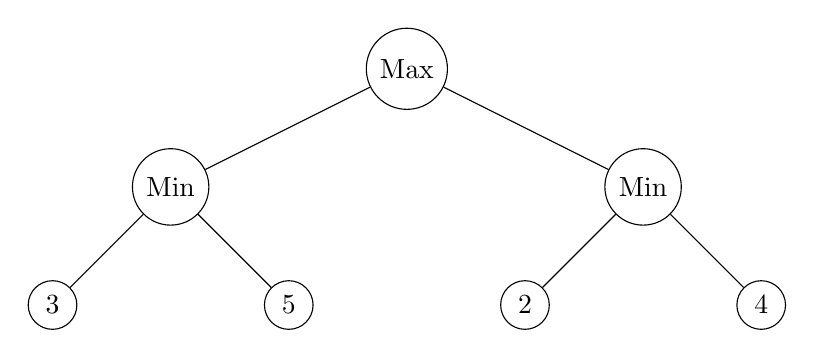
\begin{tikzpicture}[
		level distance=1.5cm,
		level 1/.style={sibling distance=6cm},
		level 2/.style={sibling distance=3cm},
		every node/.style={circle, draw, align=center}
		]
		\node {Max}
		child {node {Min}
			child {node {3}}
			child {node {5}}
		}
		child {node {Min}
			child {node {2}}
			child {node {4}}
		};
	\end{tikzpicture}
	\caption{Ein einfacher Minimax-Suchbaum mit einer Tiefe von 2.}
	\label{fig:minimax-example}
\end{figure}

\subsection*{Erklärung des Suchbaums}

Der Suchbaum in Abbildung \ref{fig:minimax-example} zeigt die Schritte des Minimax-Algorithmus:

\begin{enumerate}
	\item \textbf{Blattebene:} Die unterste Ebene enthält die Bewertungen der möglichen Endzustände aus Sicht des Max-Spielers. Diese Werte könnten durch eine Bewertungsfunktion ermittelt worden sein.
	\begin{itemize}
		\item Die Knoten haben die Werte 3, 5, 2 und 4.
	\end{itemize}
	
	\item \textbf{Min-Ebene:} Der Min-Spieler versucht, die Bewertung zu minimieren. Für jeden Min-Knoten wird der niedrigste Wert seiner Kindknoten ausgewählt:
	\begin{itemize}
		\item Der linke Min-Knoten wählt $\min(3, 5) = 3$.
		\item Der rechte Min-Knoten wählt $\min(2, 4) = 2$.
	\end{itemize}
	
	\item \textbf{Max-Ebene:} Der Max-Spieler versucht, die Bewertung zu maximieren. Der Max-Knoten wählt den höchsten Wert aus den zurückgegebenen Bewertungen der Min-Knoten:
	\begin{itemize}
		\item Der Max-Knoten wählt $\max(3, 2) = 3$.
	\end{itemize}
\end{enumerate}

\subsection*{Optimale Entscheidung}

Der optimale Zug für den Max-Spieler ist derjenige, der zu einer Bewertung von \textbf{3} führt.

\subsection*{Zusammenfassung}

Der Minimax-Algorithmus analysiert den Baum von unten nach oben:
\begin{itemize}
	\item Min-Knoten repräsentieren die Entscheidungen des Gegners (Minimierer).
	\item Max-Knoten repräsentieren die Entscheidungen des Spielers (Maximierer).
\end{itemize}

Durch diese systematische Analyse findet der Algorithmus den besten Zug für den Maximierer unter der Annahme, dass der Minimierer optimal spielt.



\section{AlphaBeta-Algorithmus}

Der Alpha-Beta-Algorithmus ist eine Optimierung des Minimax-Algorithmus, die dessen Effizienz erheblich steigert. Durch das gezielte Verwerfen von Spielzügen, die für die Entscheidung irrelevant sind, reduziert der Alpha-Beta-Algorithmus die Anzahl der bewerteten Knoten im Spielbaum. Diese Technik ist besonders wertvoll bei ressourcenbeschränkten Systemen wie einem LEGO Spike Roboter, der begrenzte Rechenleistung zur Verfügung hat.

Der Alpha-Beta-Algorithmus führt die gleichen Berechnungen wie der Minimax-Algorithmus durch, ergänzt jedoch zwei zusätzliche Parameter, Alpha und Beta, um unnötige Berechnungen zu vermeiden:

\begin{itemize}
	\item \textbf{Alpha}: Der aktuelle maximale Wert, den der Maximierer sicher erreichen kann.
	\item \textbf{Beta}: Der aktuelle minimale Wert, den der Minimierer sicher erreichen kann.
\end{itemize}

Während der Traversierung des Spielbaums werden Äste abgeschnitten, die keine Auswirkungen auf die endgültige Entscheidung haben (\textit{Pruning}). Dies geschieht, wenn:
\begin{itemize}
	\item Ein Knoten einen Wert liefert, der schlechter ist als der bisher bekannte Alpha-Wert für den Maximierer.
	\item Ein Knoten einen Wert liefert, der schlechter ist als der bisher bekannte Beta-Wert für den Minimierer.
\end{itemize}

Die Anwendung des Alpha-Beta-Algorithmus auf "Vier Gewinnt" bietet mehrere Vorteile:
\begin{itemize}
	\item \textbf{Effizienz}: Der Algorithmus reduziert die Anzahl der Knoten, die bewertet werden müssen, erheblich. Dies ermöglicht die Analyse tieferer Spielbäume mit derselben Rechenleistung.
	\item \textbf{Flexibilität}: Der Algorithmus kann leicht an die spezifische Bewertungsfunktion von "Vier Gewinnt" angepasst werden, z. B. zur Bewertung von Reihen, Spalten und Diagonalen.
	\item \textbf{Optimierung für begrenzte Ressourcen}: Ein LEGO Spike Roboter hat begrenzte Rechen- und Speicherkapazitäten. Der Alpha-Beta-Algorithmus ermöglicht es, in Echtzeit Züge zu berechnen, ohne den Roboter zu überlasten.
\end{itemize}

\section*{Beispiel: Alpha-Beta-Suchbaum}

Im Folgenden wird ein einfacher Suchbaum dargestellt, der die Funktionsweise des Alpha-Beta-Algorithmus illustriert. Der Baum zeigt, wie bestimmte Zweige (\textit{Pruning}) abgeschnitten werden, um die Effizienz zu erhöhen.

\subsection*{Suchbaum mit Alpha-Beta-Pruning}

\begin{figure}[h!]
	\centering
	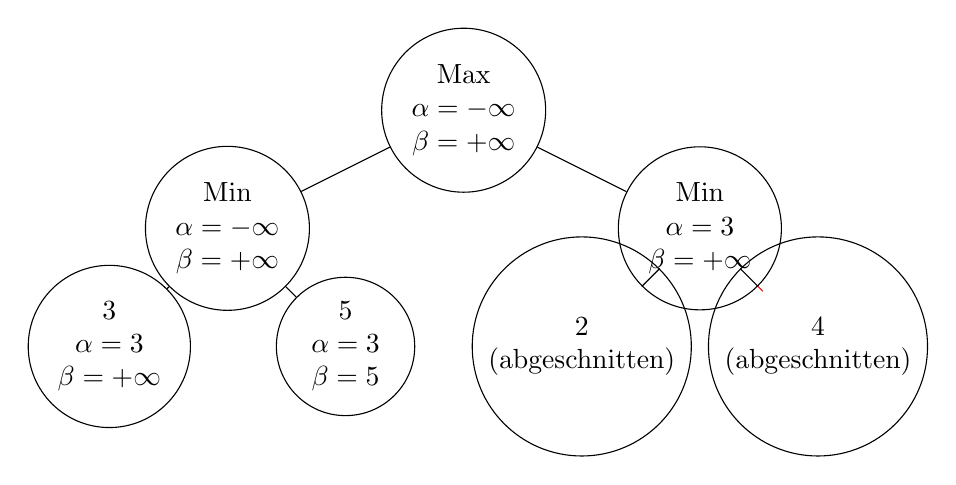
\begin{tikzpicture}[
		level distance=1.5cm,
		level 1/.style={sibling distance=6cm},
		level 2/.style={sibling distance=3cm},
		every node/.style={circle, draw, align=center}
		]
		% Root level (Max)
		\node (A) {Max\\$\alpha = -\infty$\\$\beta = +\infty$}
		% Left subtree (Min)
		child {node (B) {Min\\$\alpha = -\infty$\\$\beta = +\infty$}
			child {node {3\\$\alpha = 3$\\$\beta = +\infty$}}
			child {node {5\\$\alpha = 3$\\$\beta = 5$}}
		}
		% Right subtree (Min)
		child {node (C) {Min\\$\alpha = 3$\\$\beta = +\infty$}
			child {node {2\\(abgeschnitten)}}
			child {node {4\\(abgeschnitten)}}
		};
		% Pruning lines
		\draw[dashed, red] (C) -- +(0.8,-0.8);
	\end{tikzpicture}
	\caption{Ein Alpha-Beta-Suchbaum mit Pruning. Zweige werden abgeschnitten, wenn sie die Grenzen von Alpha und Beta verletzen.}
	\label{fig:alphabeta-example}
\end{figure}

\subsection*{Erklärung des Suchbaums}

Der Suchbaum in Abbildung \ref{fig:alphabeta-example} zeigt die Schritte des Alpha-Beta-Algorithmus:

\begin{enumerate}
	\item \textbf{Initialisierung:} Die Alpha- und Beta-Werte werden am Wurzelknoten initialisiert:
	\begin{itemize}
		\item $\alpha = -\infty$: Das beste Ergebnis, das der Maximierer bisher erreicht hat.
		\item $\beta = +\infty$: Das schlechteste Ergebnis, das der Minimierer dem Maximierer erlauben würde.
	\end{itemize}
	
	\item \textbf{Linker Teilbaum:} 
	\begin{itemize}
		\item Der Maximierer überprüft den linken Teilbaum, in dem der Minimierer aktiv ist.
		\item Der Min-Knoten prüft seine Kindknoten:
		\begin{itemize}
			\item Der erste Kindknoten liefert den Wert 3. Der Alpha-Wert wird aktualisiert: $\alpha = 3$.
			\item Der zweite Kindknoten liefert den Wert 5. Da 5 größer ist, bleibt $\alpha = 3$ bestehen.
		\end{itemize}
	\end{itemize}
	
	\item \textbf{Rechter Teilbaum (Pruning):}
	\begin{itemize}
		\item Der Maximierer prüft den rechten Teilbaum. Der Min-Knoten beginnt mit der Analyse.
		\item Bereits beim ersten Kindknoten erkennt der Algorithmus, dass dessen Wert (2) kleiner ist als $\alpha = 3$.
		\item Alle verbleibenden Kindknoten des rechten Teilbaums werden abgeschnitten (\textit{Pruning}), da sie keinen besseren Wert liefern können.
	\end{itemize}
\end{enumerate}

\subsection*{Vorteile des Alpha-Beta-Algorithmus}

Durch das Alpha-Beta-Pruning werden unnötige Berechnungen vermieden:
\begin{itemize}
	\item Der Algorithmus durchsucht nur jene Zweige, die potenziell zu besseren Ergebnissen führen.
	\item In diesem Beispiel werden zwei Knoten (Wert 2 und 4 im rechten Teilbaum) nicht berechnet.
	\item Dies erhöht die Effizienz und ermöglicht es, tiefere Suchbäume mit derselben Rechenleistung zu analysieren.
\end{itemize}